\documentclass[tikz,border=10pt]{standalone}
\usepackage{amsmath}
\usepackage{amssymb}
\usepackage{tikz}
\usetikzlibrary{arrows.meta,calc}

\definecolor{figazul}{RGB}{2,132,199}
\definecolor{figrojo}{RGB}{220,38,38}
\definecolor{figverde}{RGB}{22,163,74}

\begin{document}
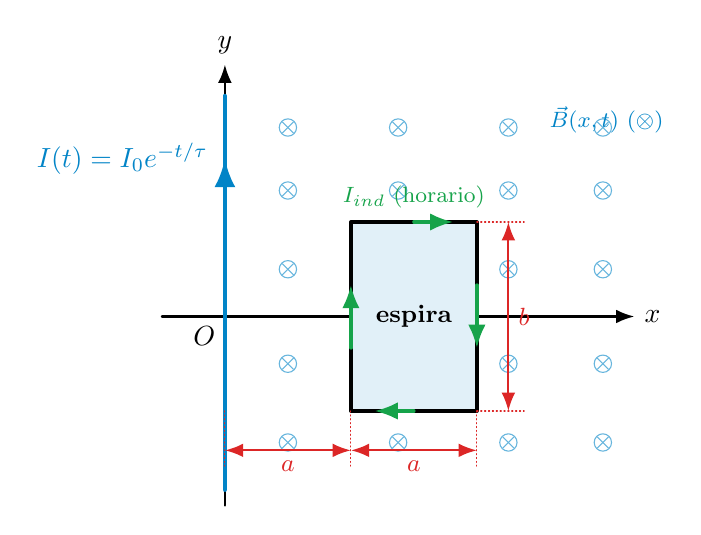
\begin{tikzpicture}[>=Latex, line cap=round, line join=round]
  % Ejes coordenados x, y
  \draw[->, thick] (-0.8, 0) -- (5.2, 0) node[right] {$x$};
  \draw[->, thick] (0, -2.4) -- (0, 3.2) node[above] {$y$};
  \node[below left] at (0,0) {$O$};

  % Cable conductor infinito sobre el eje y con corriente I(t) hacia +y
  \draw[ultra thick, color=figazul] (0, -2.2) -- (0, 2.8);
  \draw[->, ultra thick, color=figazul] (0, 1.0) -- (0, 2.0) node[left=2pt, color=figazul] {$I(t) = I_0 e^{-t/\tau}$};

  % Grilla regular de campo magnético entrante B (\otimes) en x > 0
  \foreach \gx in {0.8, 2.2, 3.6, 4.8} {
    \foreach \gy in {-1.6, -0.6, 0.6, 1.6, 2.4} {
      \draw[thin, color=figazul!60] (\gx, \gy) circle (0.11);
      \draw[thin, color=figazul!60] (\gx-0.07, \gy-0.07) -- (\gx+0.07, \gy+0.07);
      \draw[thin, color=figazul!60] (\gx-0.07, \gy+0.07) -- (\gx+0.07, \gy-0.07);
    }
  }
  \node[right, font=\footnotesize, color=figazul] at (4.0, 2.5) {$\vec{B}(x,t)$ ($\otimes$)};

  % Rectángulo conductor fijo de lados a x b
  % x va de a = 1.6 a 2a = 3.2 (ancho a = 1.6)
  % y va de -1.2 a +1.2 (altura b = 2.4)
  \draw[very thick, fill=figazul!12] (1.6, -1.2) rectangle (3.2, 1.2);
  \node[font=\small\bfseries] at (2.4, 0) {espira};

  % Cotas en rojo
  % Cota a de distancia desde el cable al borde izquierdo
  \draw[<->, thick, color=figrojo] (0, -1.7) -- (1.6, -1.7) node[midway, below, color=figrojo, font=\small] {$a$};
  \draw[densely dotted, thin, color=figrojo] (1.6, -1.2) -- (1.6, -1.9);
  \draw[densely dotted, thin, color=figrojo] (0, -1.2) -- (0, -1.9);

  % Cota a del ancho del rectángulo
  \draw[<->, thick, color=figrojo] (1.6, -1.7) -- (3.2, -1.7) node[midway, below, color=figrojo, font=\small] {$a$};
  \draw[densely dotted, thin, color=figrojo] (3.2, -1.2) -- (3.2, -1.9);

  % Cota b de la altura del rectángulo
  \draw[<->, thick, color=figrojo] (3.6, -1.2) -- (3.6, 1.2) node[midway, right, color=figrojo, font=\small] {$b$};
  \draw[densely dotted, thin, color=figrojo] (3.2, -1.2) -- (3.8, -1.2);
  \draw[densely dotted, thin, color=figrojo] (3.2, 1.2) -- (3.8, 1.2);

  % Corriente inducida I_ind en sentido horario (según Lenz al decaer I(t))
  \draw[->, very thick, color=figverde] (2.4, 1.2) -- (2.9, 1.2);
  \draw[->, very thick, color=figverde] (3.2, 0.4) -- (3.2, -0.4);
  \draw[->, very thick, color=figverde] (2.4, -1.2) -- (1.9, -1.2);
  \draw[->, very thick, color=figverde] (1.6, -0.4) -- (1.6, 0.4);
  \node[above, font=\footnotesize, color=figverde] at (2.4, 1.25) {$I_{ind}$ (horario)};

\end{tikzpicture}
\end{document}
